\section{Modello}

\begin{frame}{Dati di precipitazione e temperatura}

  % ---------- Parte di testo ----------
  \begin{itemize}[label=$\blacktriangleright$]
    \item mappe giornaliere (periodo 1881--2023)
    \item risoluzione spaziale 30 arco-secondi
    \item ricostruzione con metodo delle anomalie
  \end{itemize}

  \vfill

  \vspace{0.5ex}
  \begin{columns}[T, onlytextwidth]
    \begin{column}{0.48\textwidth}
      \centering
      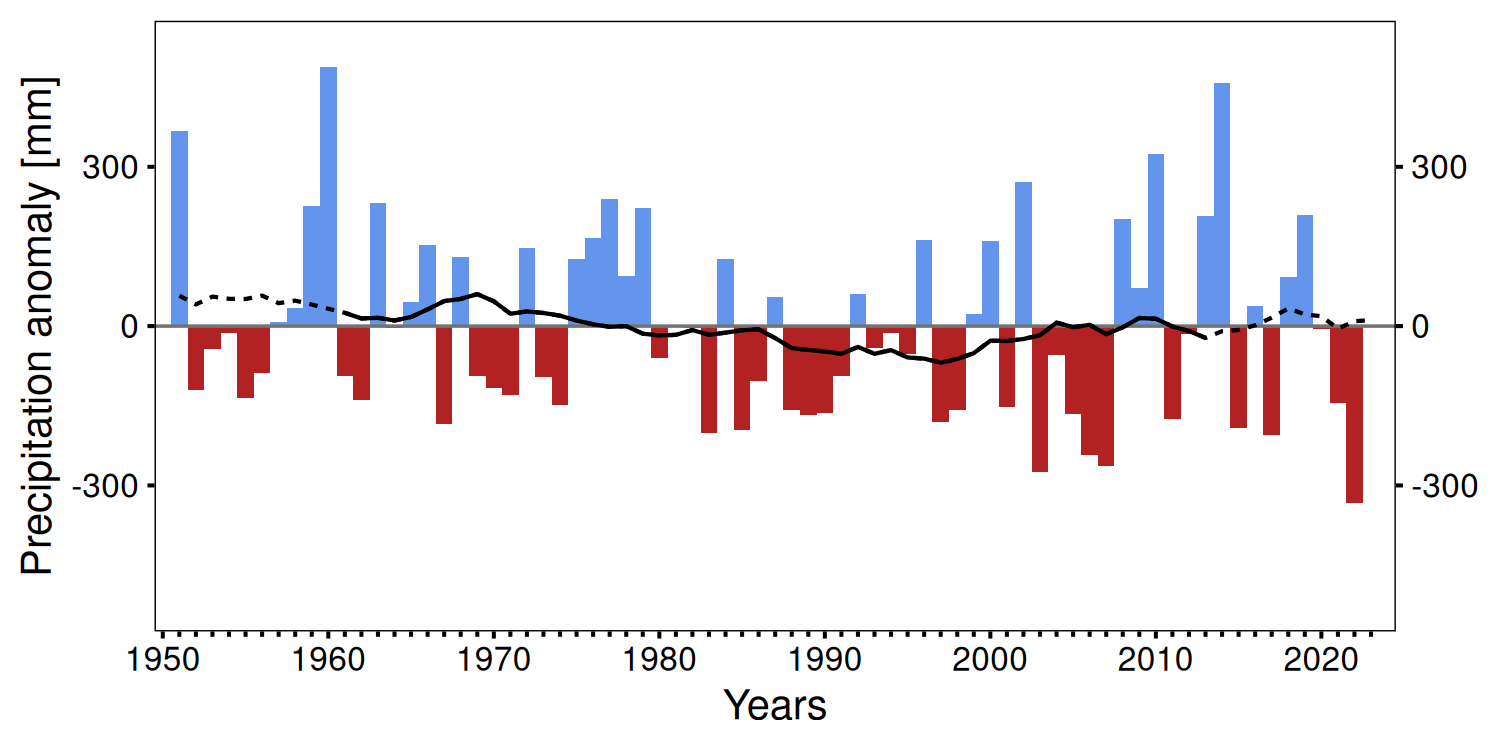
\includegraphics[width=\linewidth, height=0.5\textheight, keepaspectratio]{images/model/prec_anomaly_clima_1991_2020.png}

      \vspace{0.5ex}
      {\footnotesize Anomalia precipitazioni annuali medie}
    \end{column}

    \begin{column}{0.48\textwidth}
      \centering
      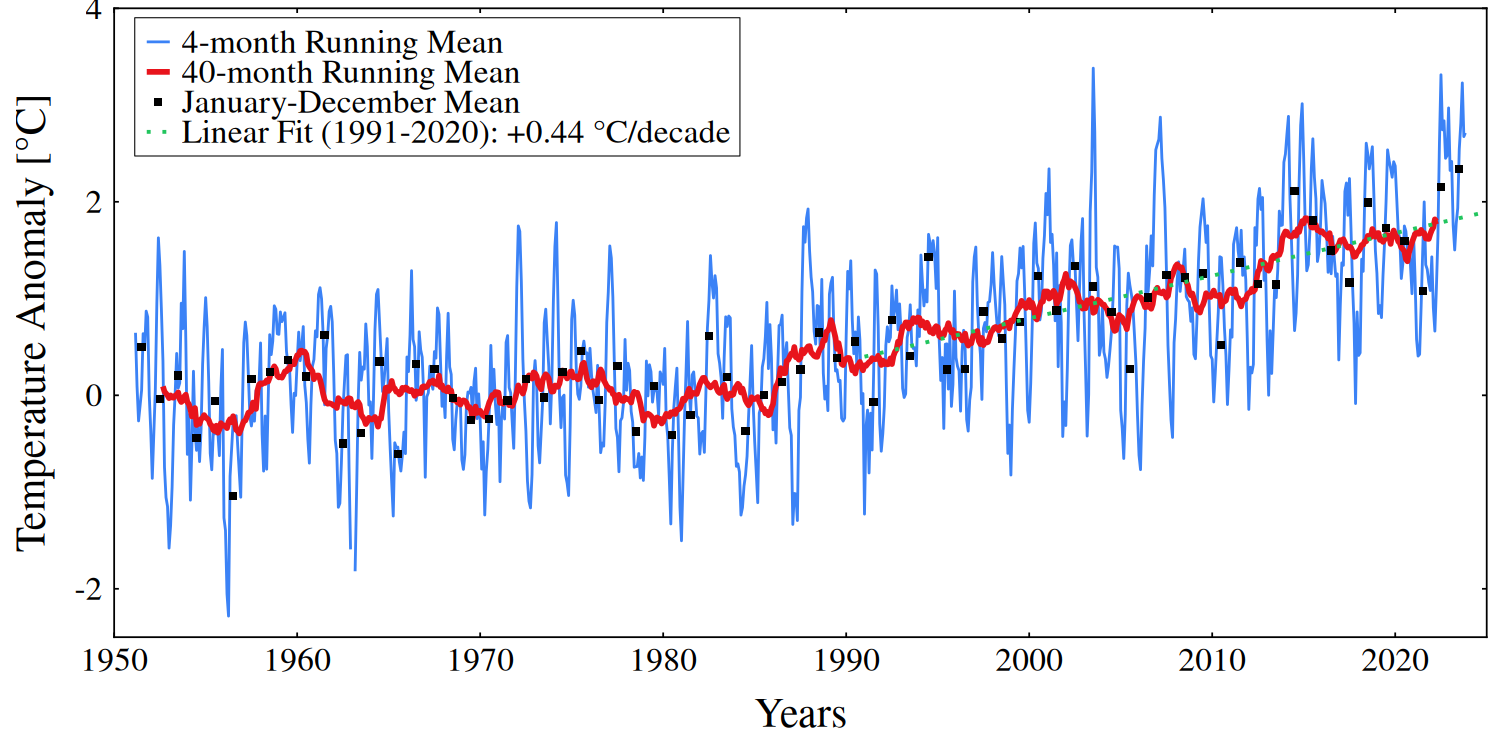
\includegraphics[width=\linewidth, height=0.5\textheight, keepaspectratio]{images/model/mean_temperature_trend.png}
      
      \vspace{0.5ex}
      {\footnotesize Evoluzione temperatura media su IH-GAR}
    \end{column}
  \end{columns}

\end{frame}